\subsection{\playlist}
    \subsubsection{\playlist の作成}
        \begin{enumerate}
            \item ホーム画面のハンバーガーメニューを表示し、\ttbox{プレイリスト}を押下してください。
                \begin{figure}[htbp]
                    \centering
                    \fbox{
                        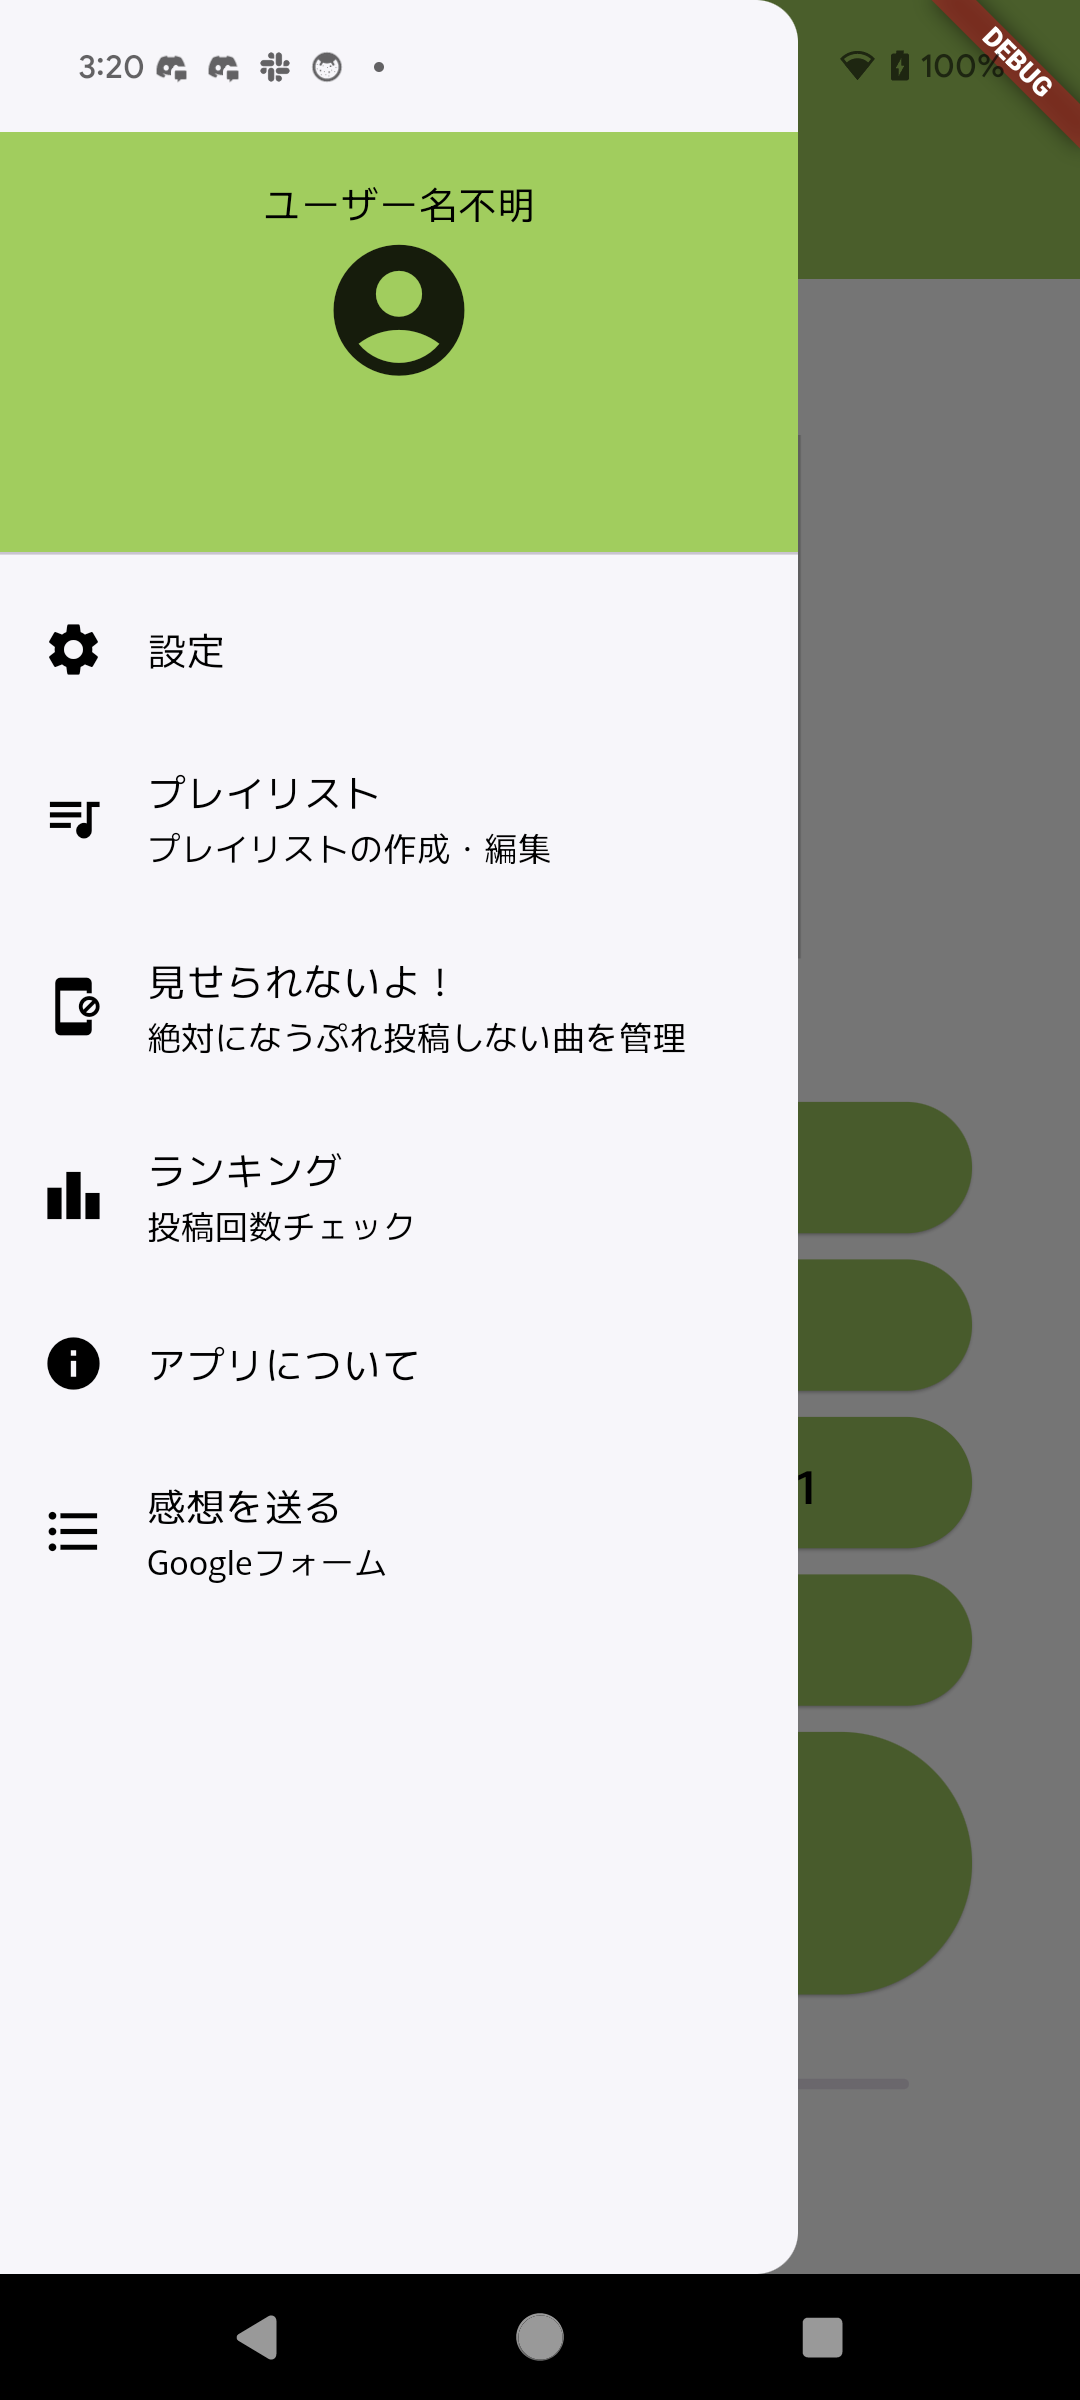
\includegraphics[width=5cm]{./pictures/playlist1.png}
                    }
                    \caption{ハンバーガーメニュー(\currentVersion)}
                    \label{img:playlist1}
                \end{figure}

            \newpage
            \item プレイリスト一覧画面の\ttbox{新規作成}を押下してプレイリスト詳細画面に移動してください。
                \begin{figure}[htbp]
                    \begin{minipage}[b]{0.45\linewidth}
                        \centering
                        \fbox{
                            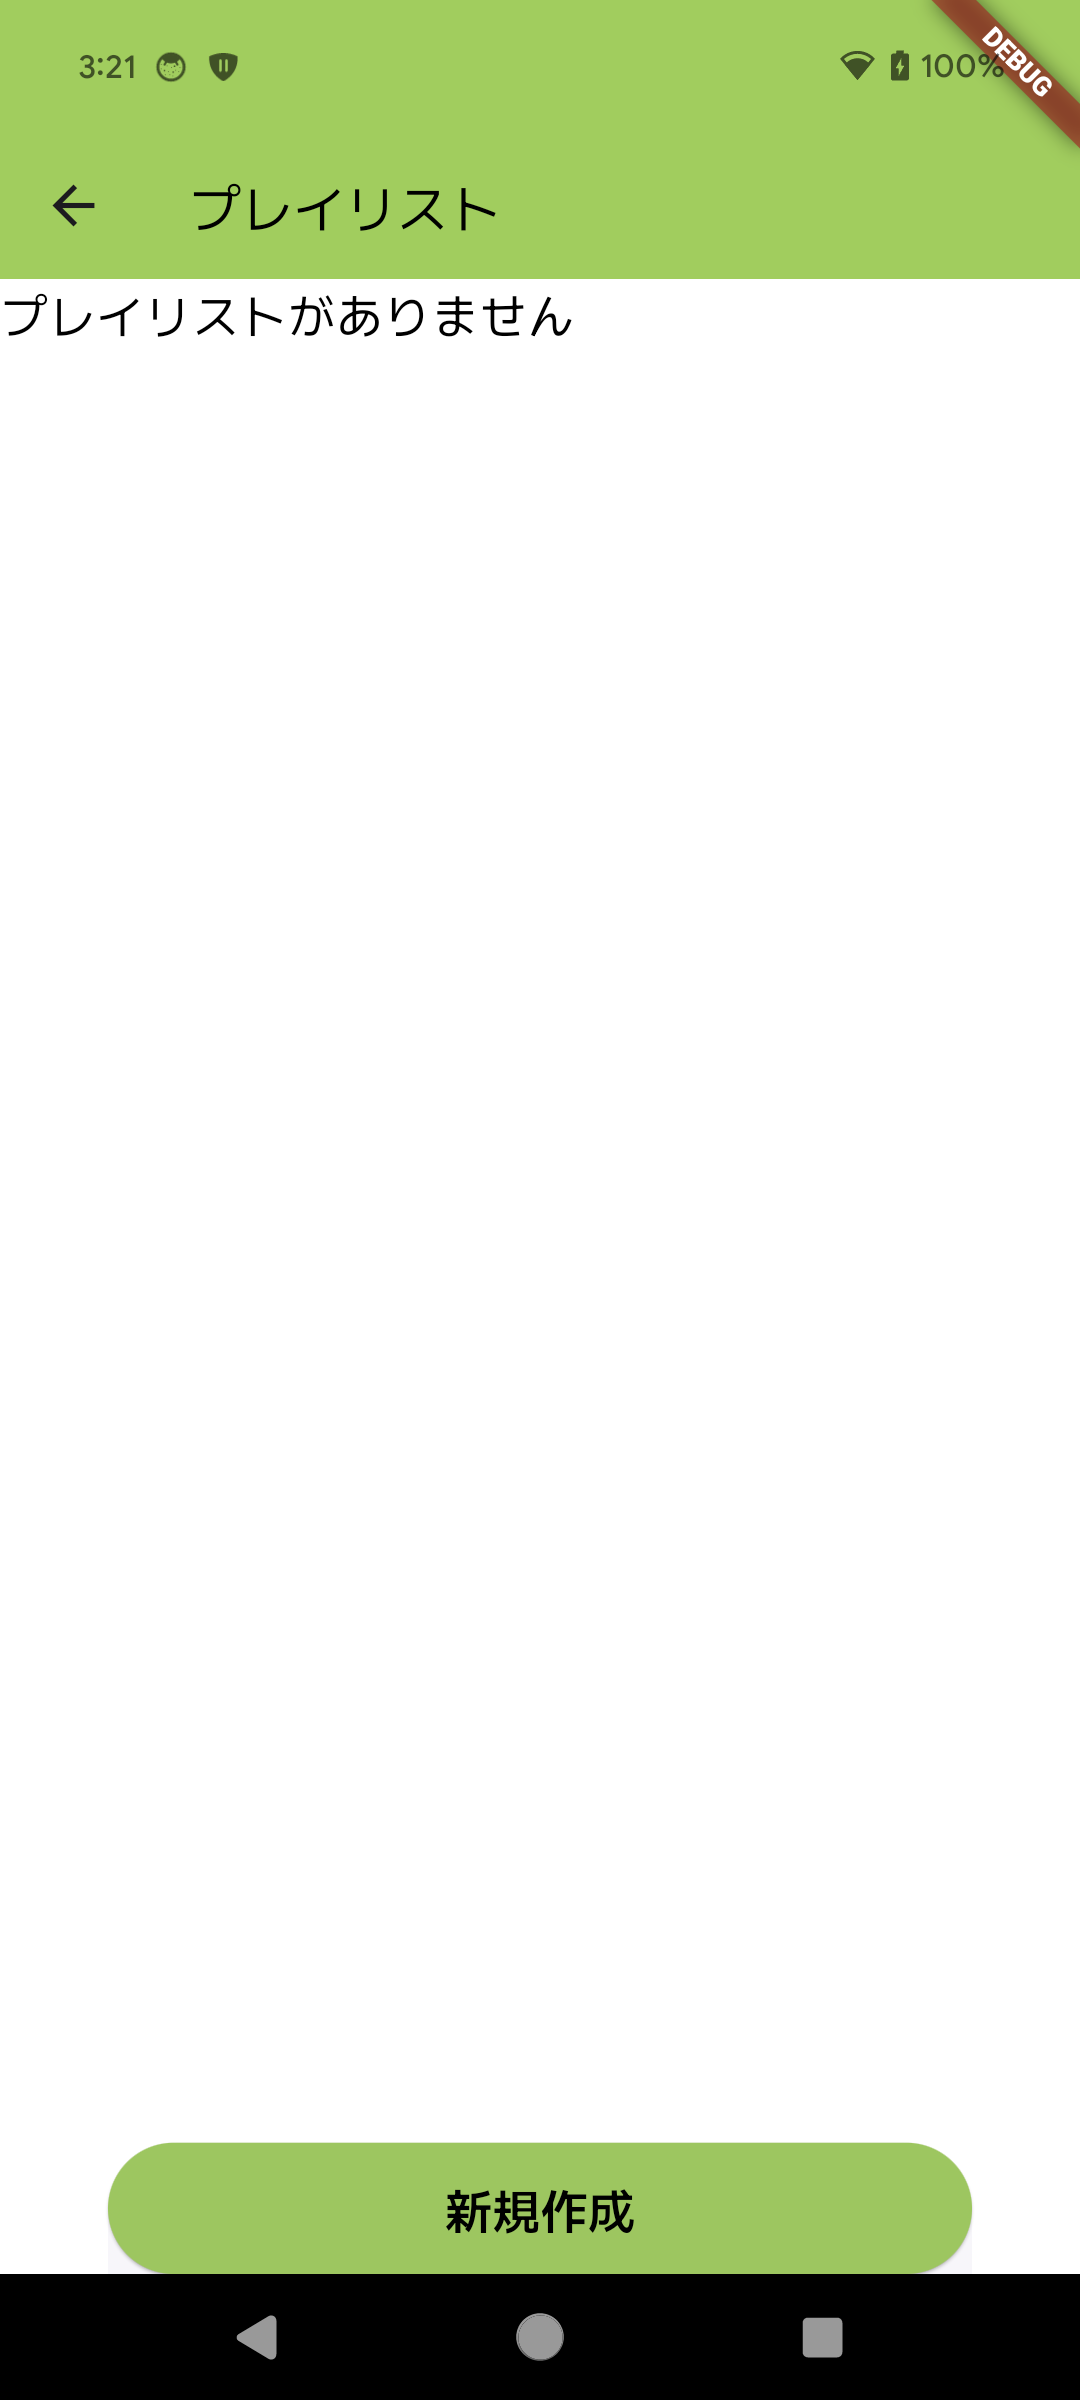
\includegraphics[width=5cm]{./pictures/playlist2.png}
                        }
                        \caption{プレイリスト一覧画面}
                        \label{img:playlist2}
                    \end{minipage}
                    \begin{minipage}[b]{0.45\linewidth}
                        \centering
                        \fbox{
                            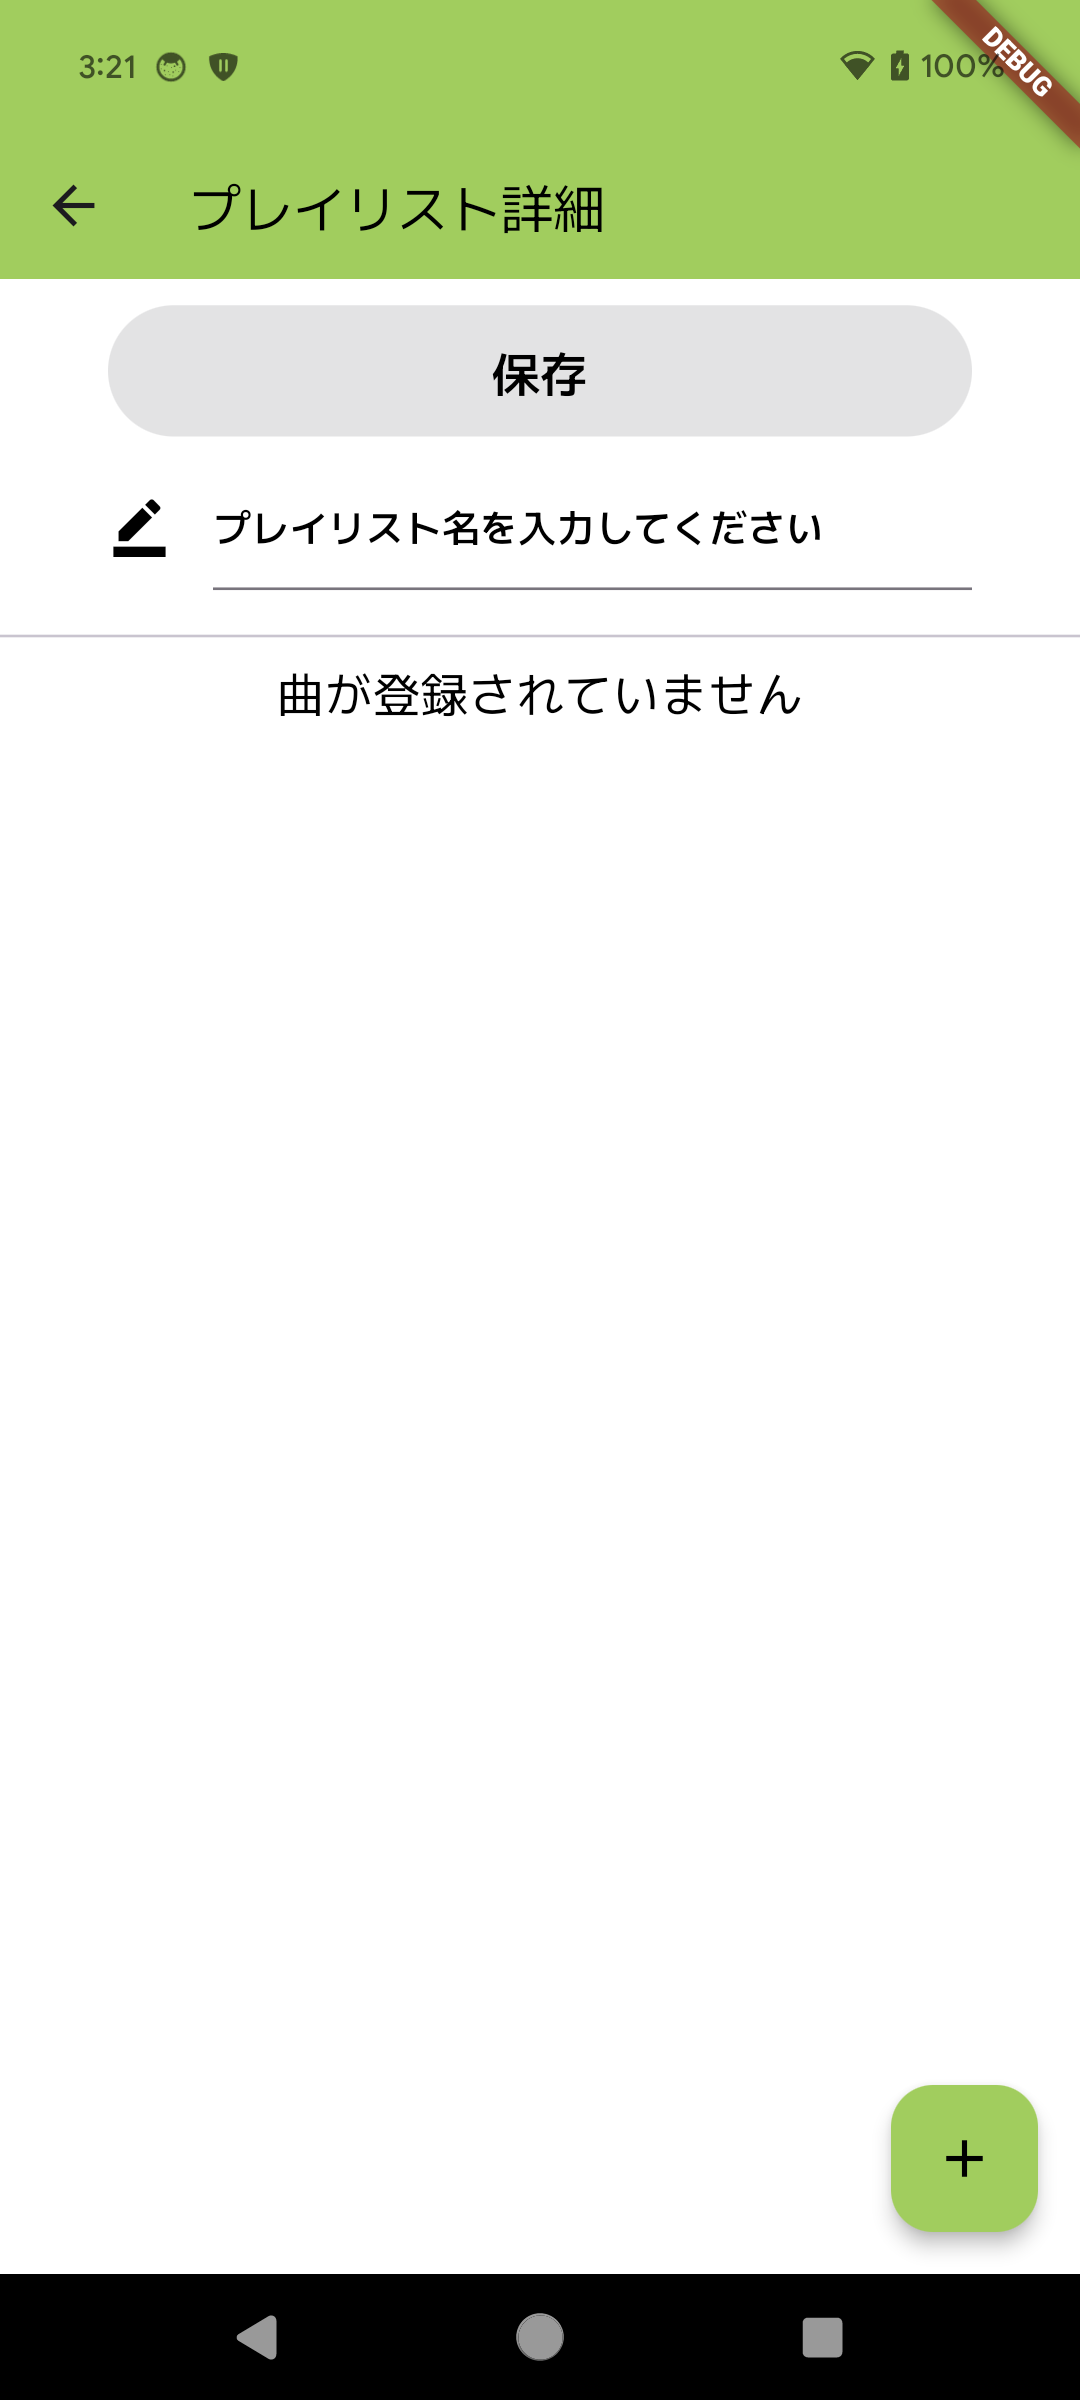
\includegraphics[width=5cm]{./pictures/playlist3.png}
                        }
                        \caption{プレイリスト詳細画面}
                        \label{img:playlist3}
                    \end{minipage}
                \end{figure}

            \newpage
            \item プレイリスト詳細画面の\ttbox{+}ボタンを押下して、登録する曲を選択してください。
                \begin{figure}[htbp]
                    \begin{minipage}[b]{0.45\linewidth}
                        \centering
                        \fbox{
                            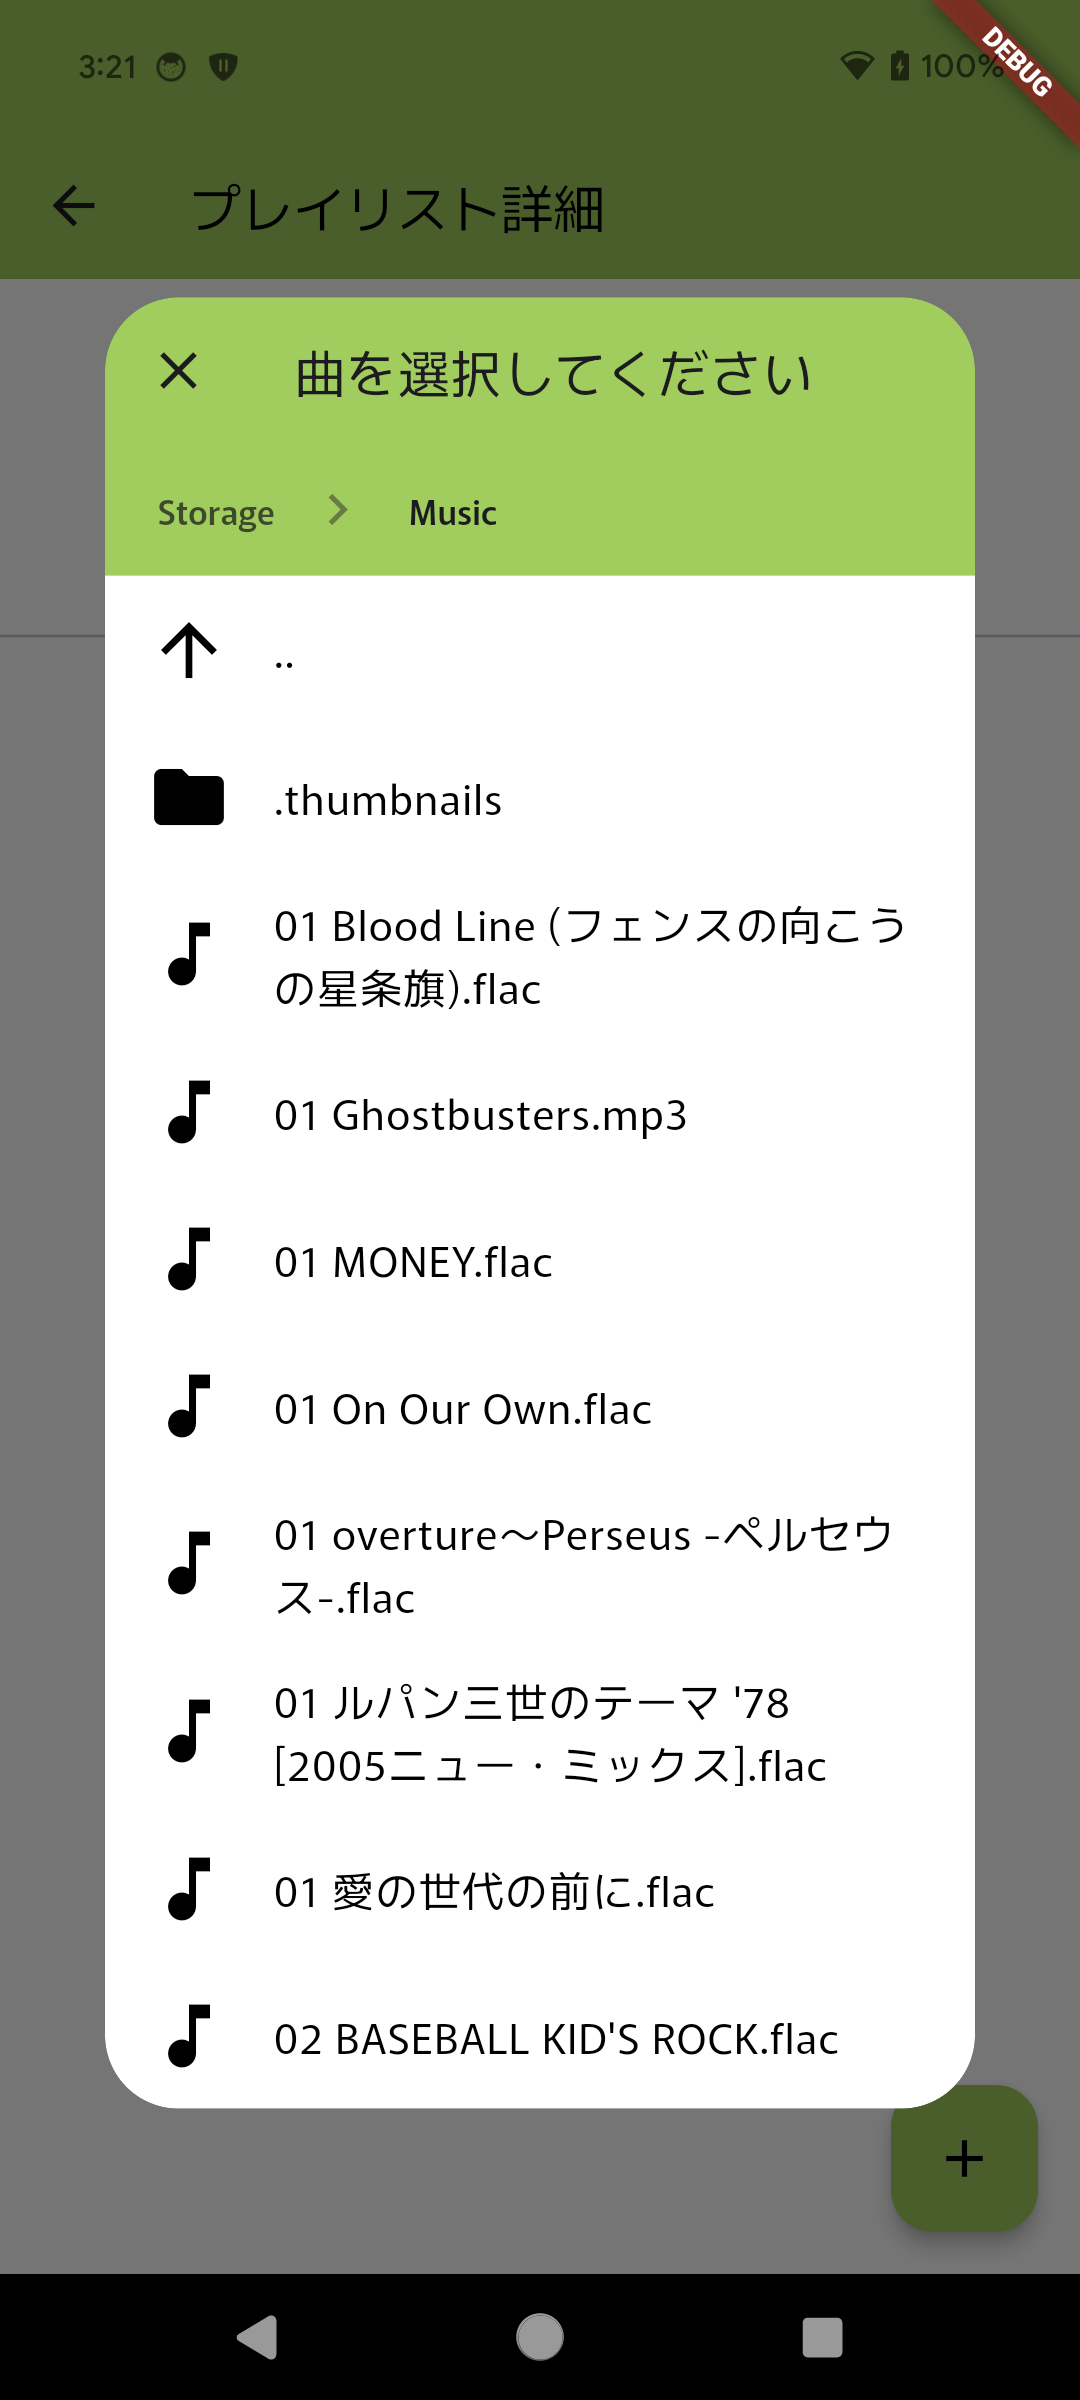
\includegraphics[width=5cm]{./pictures/playlist4.png}
                        }
                        \caption{曲選択ダイアログ}
                        \label{img:playlist4}
                    \end{minipage}
                    \begin{minipage}[b]{0.45\linewidth}
                        \centering
                        \fbox{
                            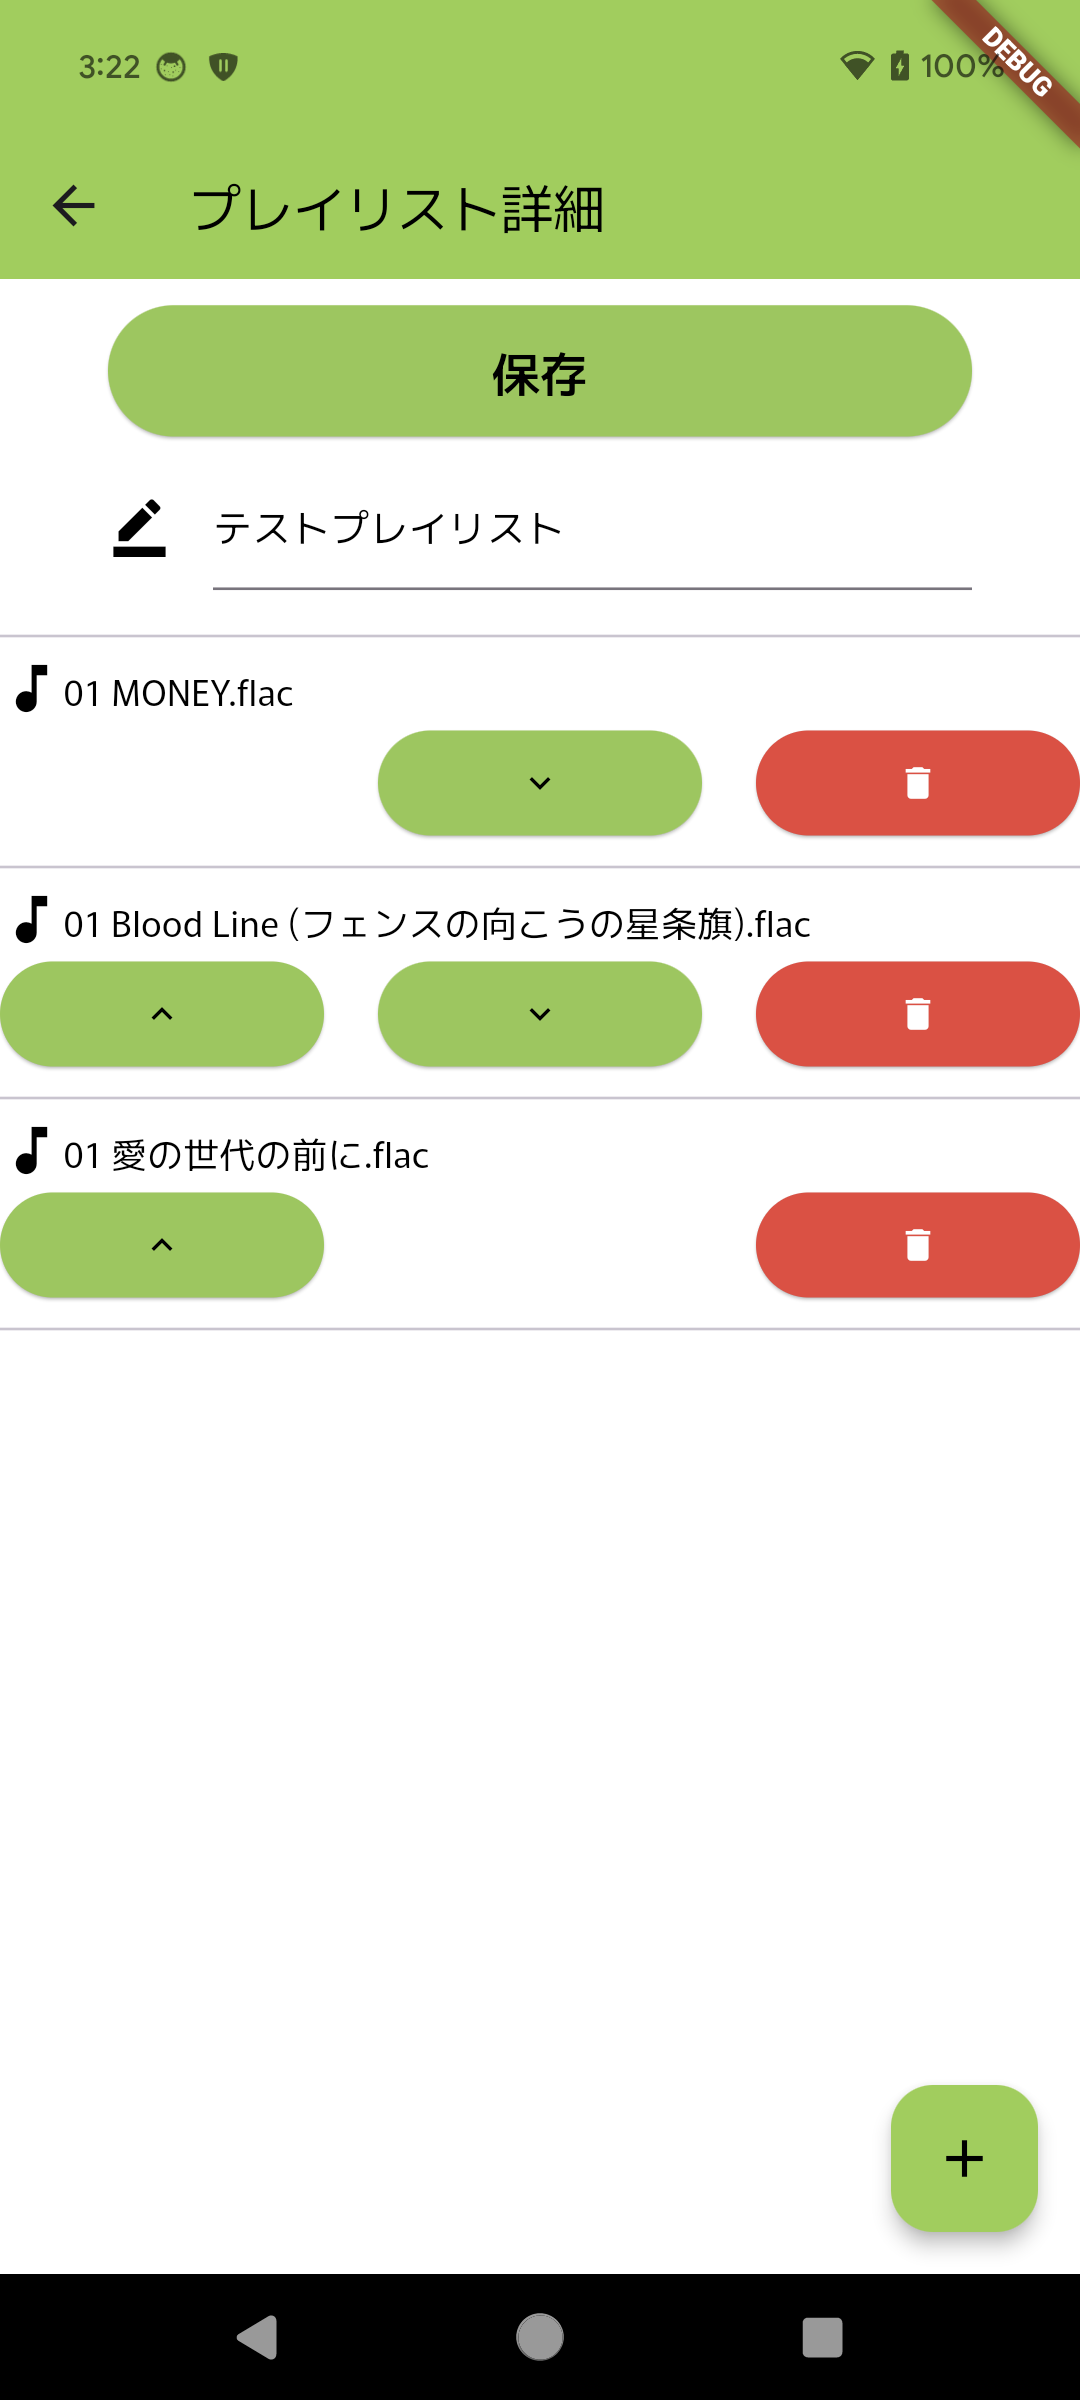
\includegraphics[width=5cm]{./pictures/playlist5.png}
                        }
                        \caption{曲登録後のプレイリスト詳細画面}
                        \label{img:playlist5}
                    \end{minipage}
                    \caption*{曲の登録(\currentVersion)}
                \end{figure}

                \begin{itemize}
                    \item \ttbox{↑}ボタンを押下すると、再生順をひとつ前に移動させることができます。
                    \item \ttbox{↓}ボタンを押下すると、再生順をひとつ後ろに移動させることができます。
                    \item ゴミ箱ボタンを押下すると、その曲をプレイリストから除外することができます。
                \end{itemize}

            \newpage
            \item 曲を登録し、プレイリスト名を入力すると\ttbox{保存}ボタンが押下できるようになるので、押下してプレイリストを保存してください。
                \begin{figure}[htbp]
                    \centering
                    \fbox{
                        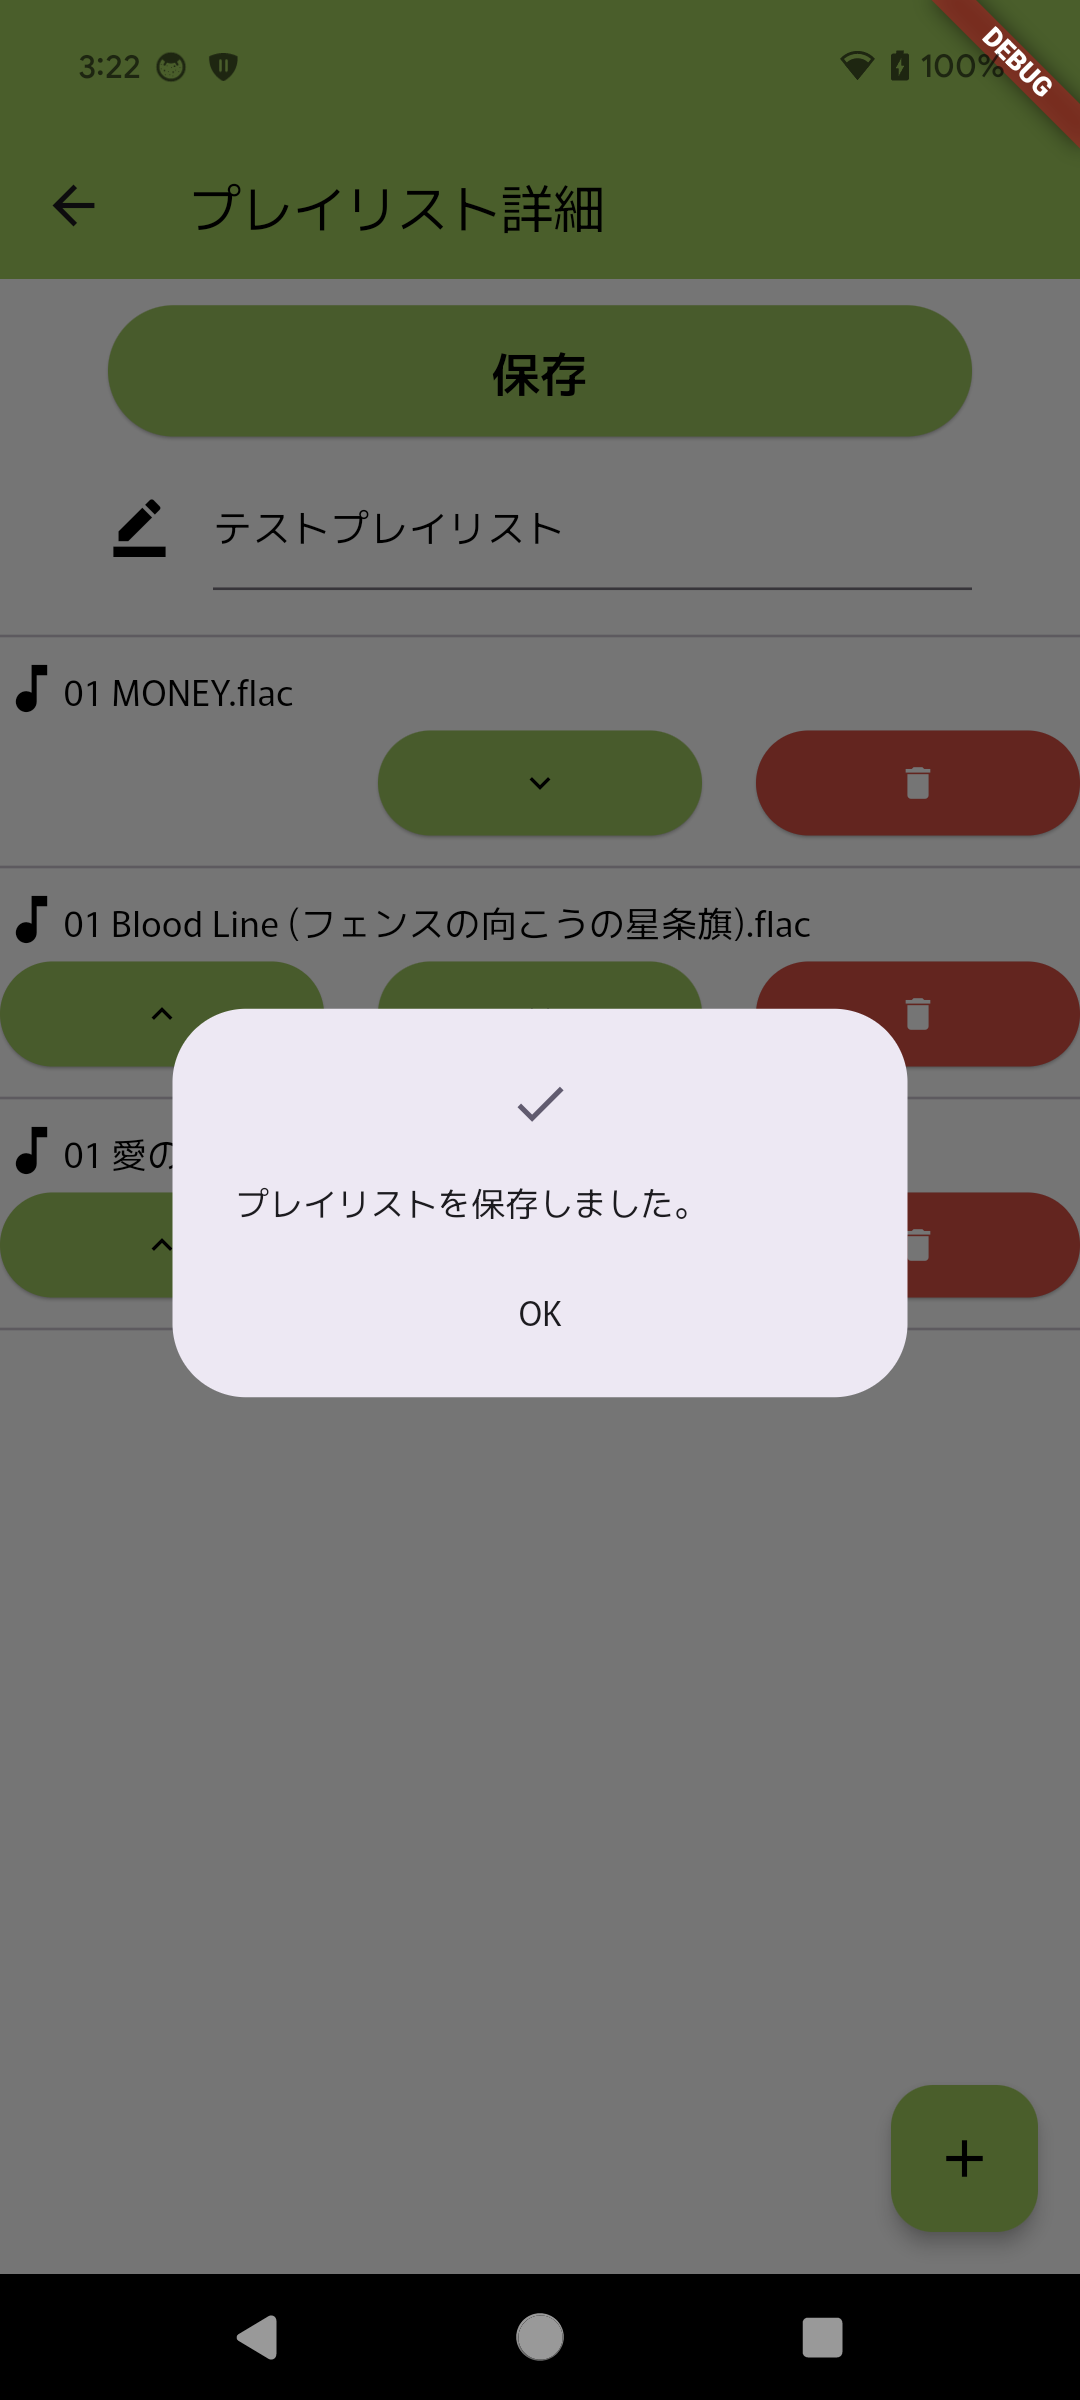
\includegraphics[width=5cm]{./pictures/playlist6.png}
                    }
                    \caption{プレイリスト保存完了ダイアログ}
                    \label{img:playlist6}
                \end{figure}

            \newpage
            \item 自動的にプレイリスト一覧画面に戻り、一覧に先ほど追加したプレイリストが追加されています。
                \begin{figure}[htbp]
                    \centering
                    \fbox{
                        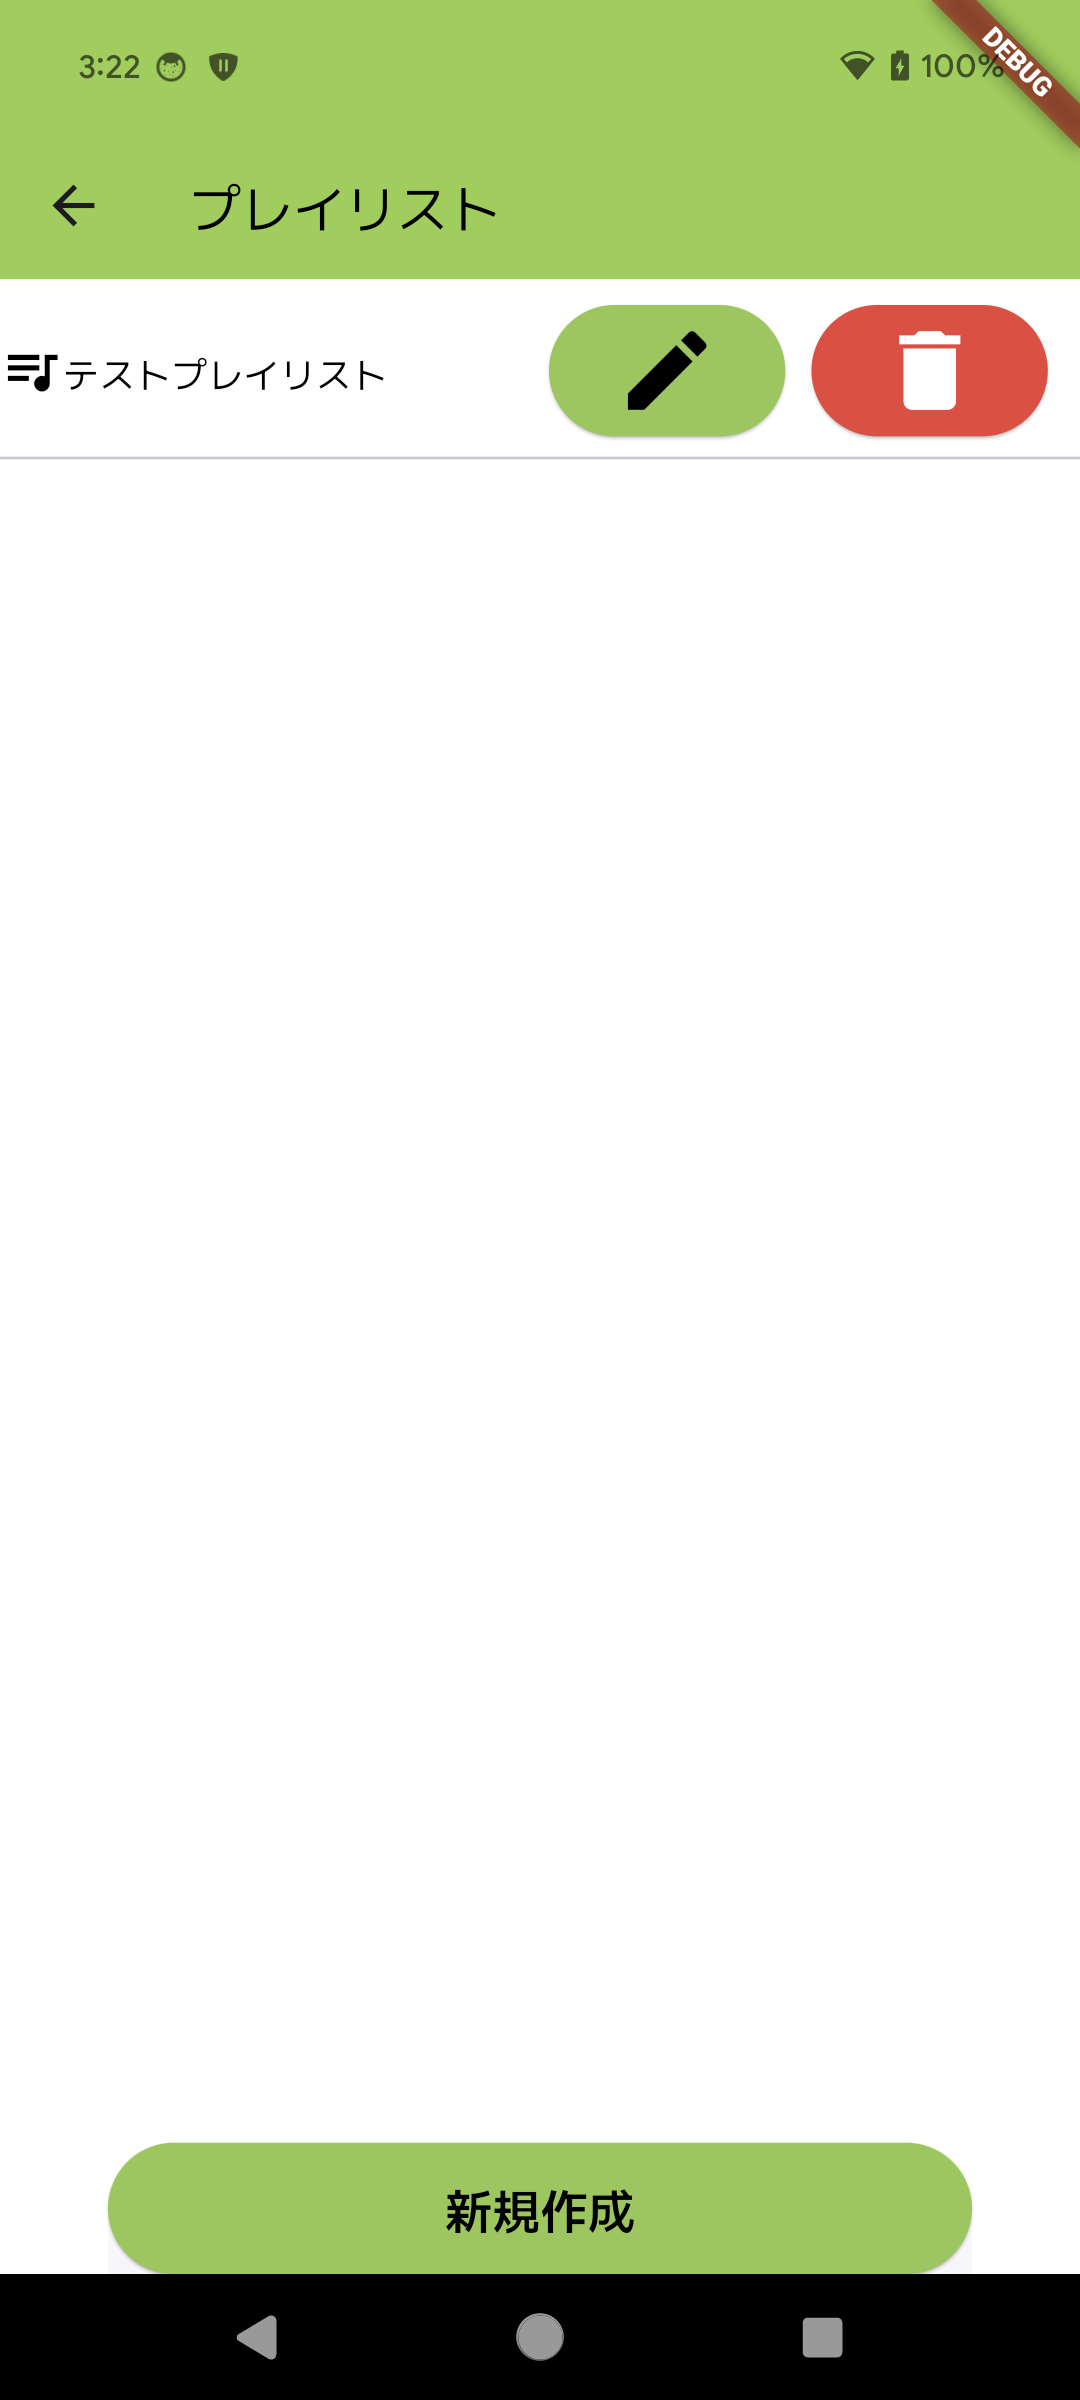
\includegraphics[width=5cm]{./pictures/playlist7.png}
                    }
                    \caption{プレイリスト作成後のプレイリスト一覧画面}
                    \label{img:playlist7}
                \end{figure}
                \begin{itemize}
                    \item 鉛筆ボタンを押下すると、既存のプレイリストを編集することができます。
                    \item ゴミ箱ボタンを押下すると、プレイリストを削除することができます。
                \end{itemize}
        \end{enumerate}

    \newpage
    \subsubsection{\playlist の再生}
        \begin{enumerate}
            \item ホーム画面の\ttbox{プレイリストを選択}ボタンを押下して、プレイリスト選択ダイアログを表示してください。
                \begin{figure}[htbp]
                    \begin{minipage}[b]{0.45\linewidth}
                        \centering
                        \fbox{
                            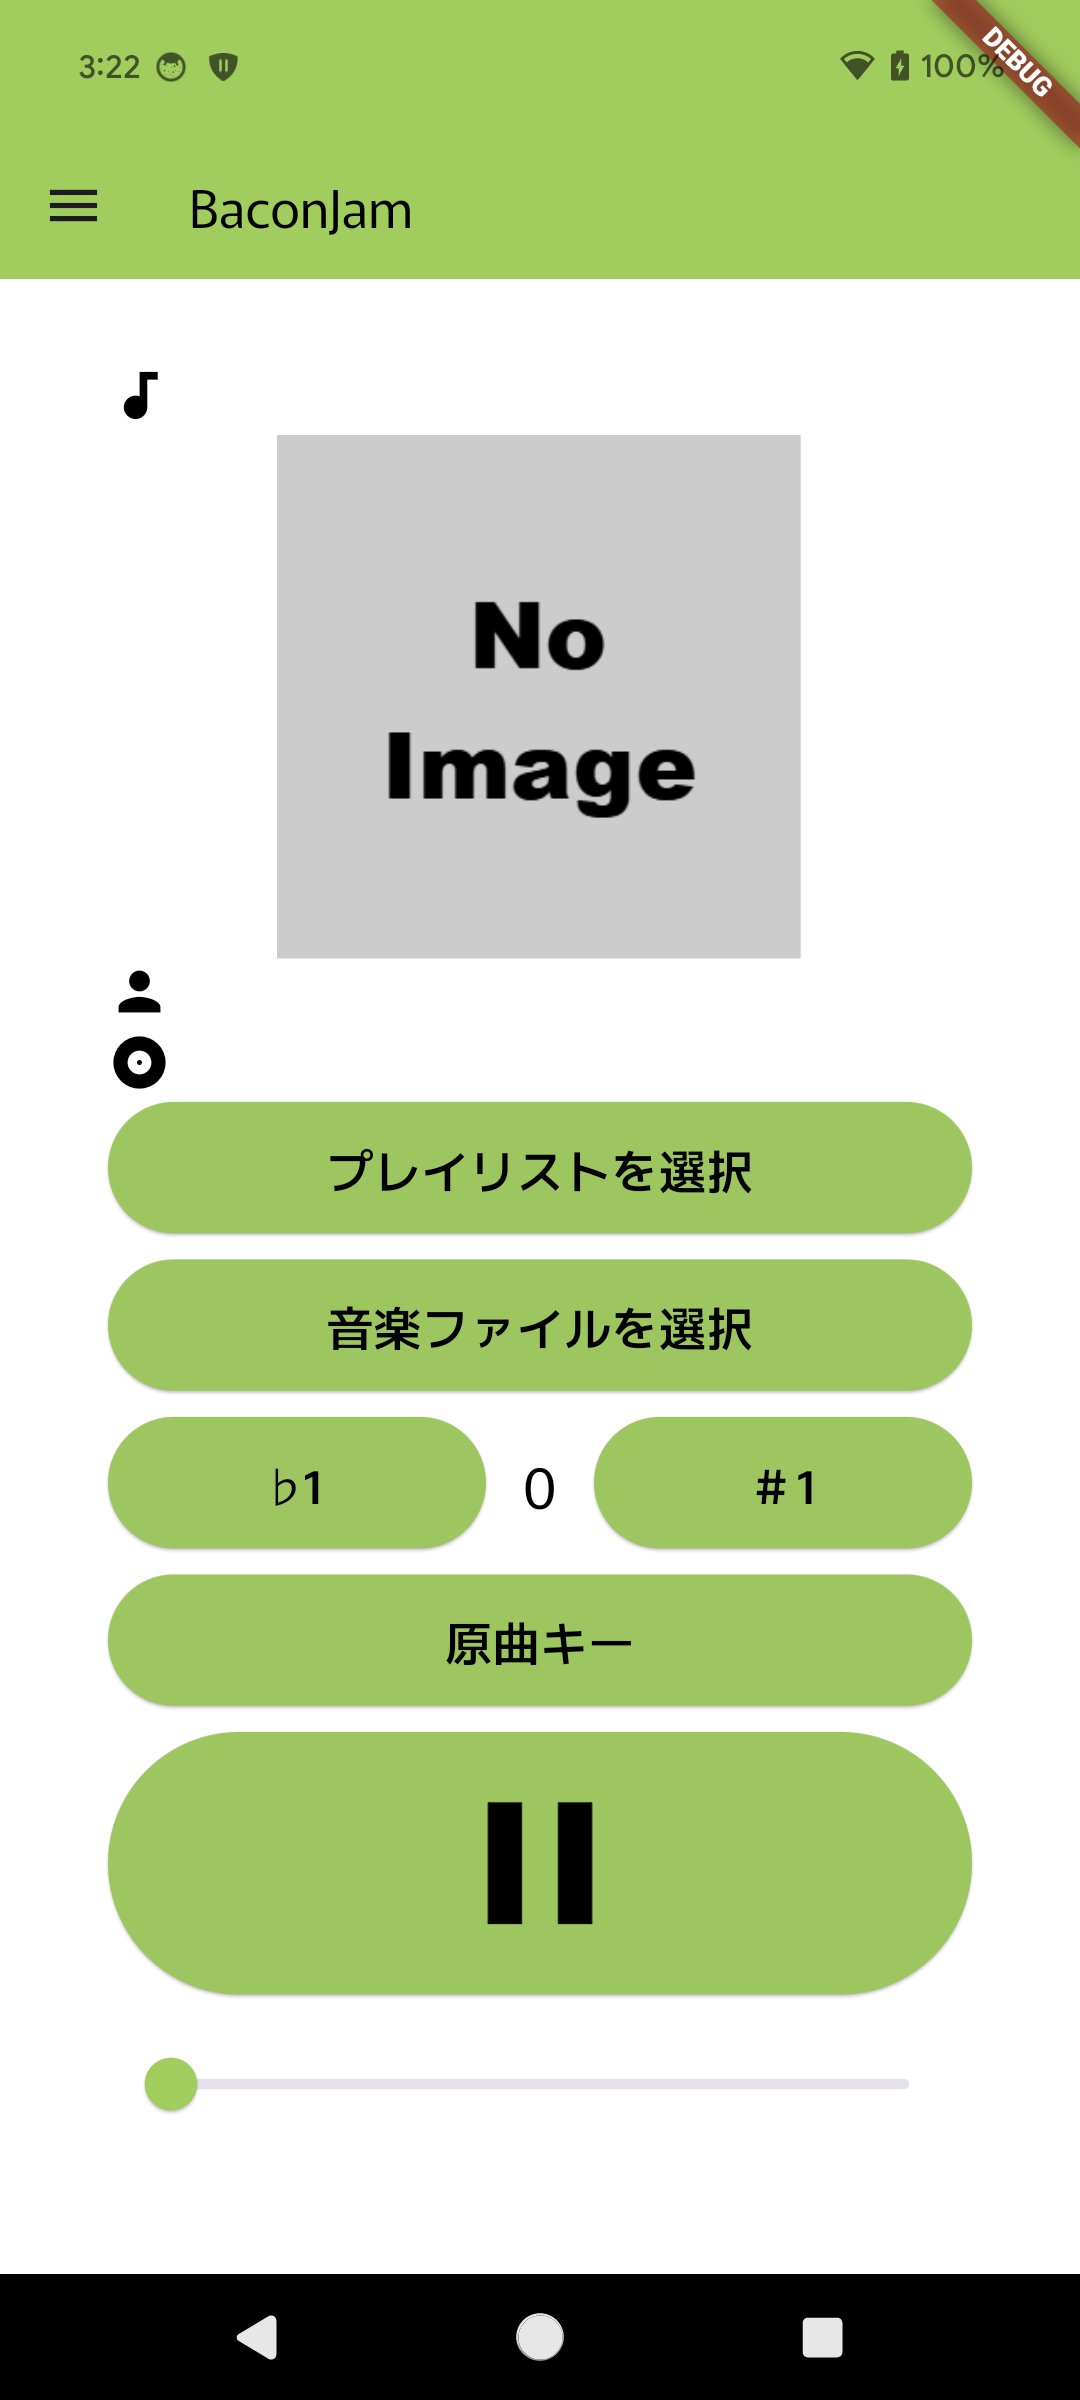
\includegraphics[width=5cm]{./pictures/playlist8.png}
                        }
                        \caption{ホーム画面}
                        \label{img:playlist8}
                    \end{minipage}
                    \begin{minipage}[b]{0.45\linewidth}
                        \centering
                        \fbox{
                            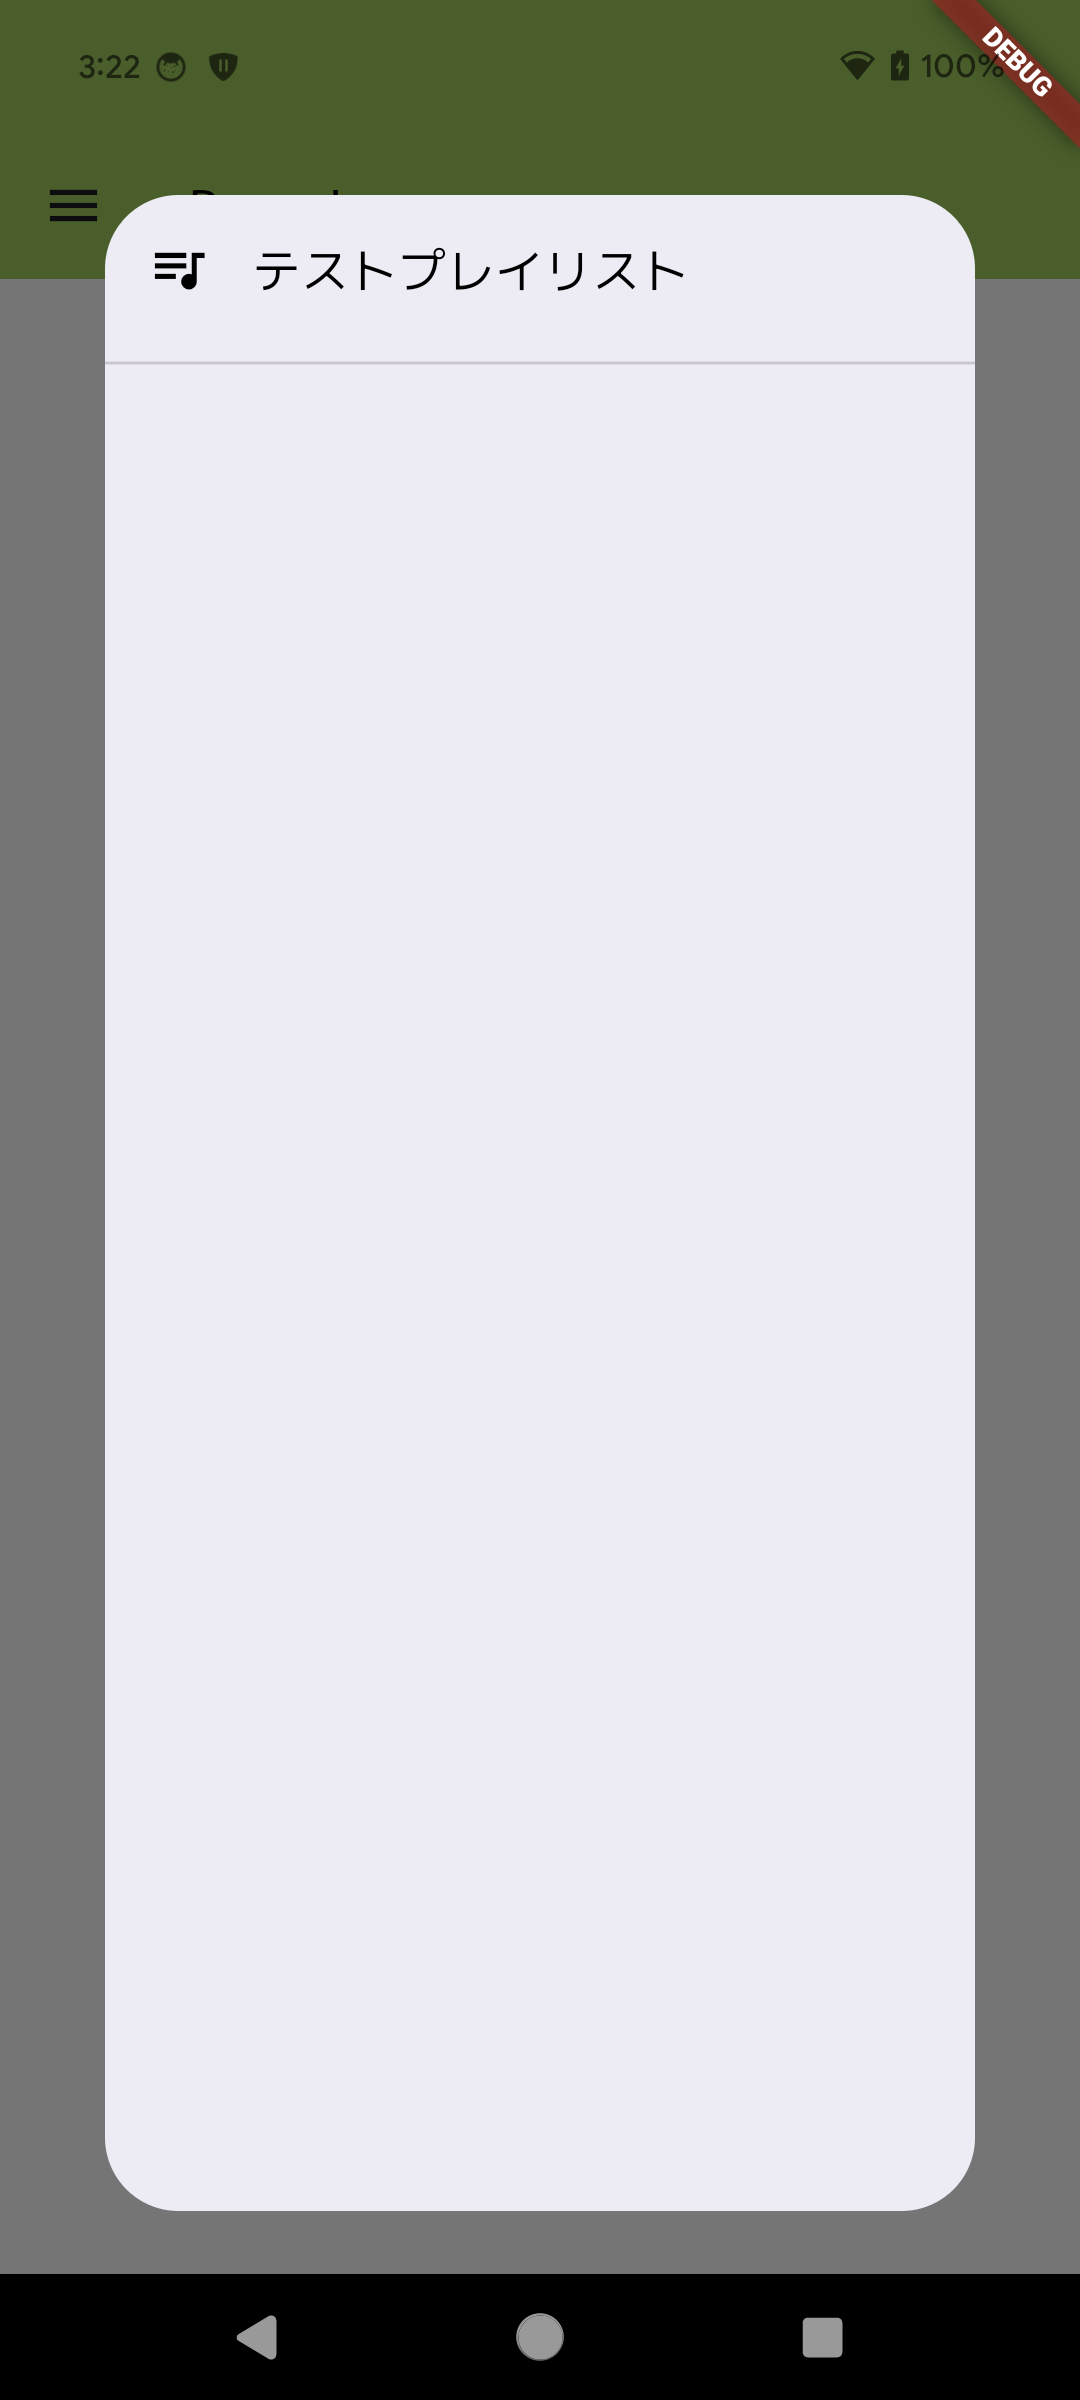
\includegraphics[width=5cm]{./pictures/playlist9.png}
                        }
                        \caption{プレイリスト選択ダイアログ}
                        \label{img:playlist9}
                    \end{minipage}
                    \caption*{プレイリストを選択(\currentVersion)}
                \end{figure}

            \newpage
            \item 再生したいプレイリスト名を押下すると、そのプレイリストに登録した曲を順に再生します。
                \begin{itemize}
                    \item プレイリスト作成後に削除された曲はスキップします。
                    \item プレイリスト内のすべての曲が削除されている場合、再生エラーを表示します。
                \end{itemize}
        \end{enumerate}